\documentclass[journal,a4paper]{IEEEtran}

\usepackage{cite}
\usepackage{booktabs}
\usepackage{amsmath}
\usepackage{amssymb}
\usepackage{url}
\usepackage{graphicx}

\newcommand{\E}{\mathbb{E}}
\newcommand{\Prb}{\mathbb{P}}
\newcommand{\R}{\mathbb{R}}
\newcommand{\ind}{\mathbb{I}}
\newcommand{\sigmoid}{\operatorname{logit}^{-1}}
\newcommand{\logit}{\operatorname{logit}}
\newcommand{\Bern}{\operatorname{Bernoulli}}
\newcommand{\Normal}{\mathcal{N}}

\begin{document}

\title{Beyond Fractional Kelly: Bayesian Metacognition, Exact AMM Execution, and Poisson Opportunities in Prediction Markets}

\author{Jan~Ol\v{s}ina, AI generated paper\\[1ex]
Independent Researcher, Prague, Czech Republic\\
email: \texttt{jan.olsina@gmail.com}, ORCID: \texttt{0009-0003-9816-3958}.}

\maketitle

\begin{abstract}
This article develops a normative decision model for an automated prediction-market trader that is uncertain about its own reasoning. Kelly optimization determines how to act on a posterior predictive distribution, but it does not determine how much a raw forecast should be trusted relative to a market. The paper therefore separates an object-level forecast from the trading agent's final Bayesian belief. The market is treated as a public-information baseline, while the agent contributes an uncertain incremental log Bayes factor. A hierarchical observation model relates this latent evidential contribution to the output and diagnostics of a fallible reasoning process; historical resolutions update interpretable reliability and failure-mode parameters rather than an unexplained stake multiplier. A shared reliability state induces portfolio dependence, while task-specific reasoning uncertainty produces endogenous shrinkage or amplification. The epistemic model is combined with exact automated-market-maker execution, signed portfolio rebalancing, expected-log wealth, and a stochastic-control model in which future opportunities arrive as a marked Poisson process. The article gives a tractable shared-slope specialization and a numerical example using the weighted geometric-mean constant-product mechanism implemented by Manifold Markets.
\end{abstract}

\begin{IEEEkeywords}
prediction markets, Kelly criterion, Bayesian metacognition, forecast aggregation, automated market maker, constant-product market maker, Poisson arrivals, stochastic control.
\end{IEEEkeywords}

\section{Introduction}
The Kelly criterion answers a decision question: given a probability model, payoffs, and available wealth, which position maximizes expected logarithmic wealth \cite{kelly1956,coverthomas2006,maclean2011}? It does not, by itself, derive the probability model. This distinction is central for an automated prediction-market agent. Such an agent must reason not only about an uncertain event, but also about whether its own inference adds information beyond the market, whether several trades share the same reasoning failure, how execution moves an automated market maker (AMM), and whether cash should be retained for later opportunities.

A common practical response is fractional Kelly: calculate a Kelly position from a point forecast and multiply it by a fixed number below one. This may be useful as an operational safeguard, but one scalar cannot generally represent task-specific reasoning uncertainty, shared model risk, nonlinear slippage, existing positions, or the option value of cash. The goal of this article is to derive these effects from a single posterior decision problem instead of imposing an exogenous fraction.

The paper makes four main contributions. First, it distinguishes a raw object-level forecast from a final meta-level Bayesian posterior. The market quote is used as a baseline and the agent's incremental information is represented by a latent log Bayes factor. Second, it models the raw reasoning output as a fallible observation of that latent evidential contribution. A hierarchical shared state captures common failures across forecasts, while task diagnostics control question-specific reliability. Third, it combines the resulting joint predictive distribution with exact AMM fills and signed position changes. Fourth, it formulates liquidity reservation as stochastic control under marked Poisson arrivals, explicitly distinguishing a hold-to-settlement arrival model from a more general impulse-control model with rebalancing.

The article proceeds as follows. Section~II develops Bayesian reasoning about the agent's own reasoning and shows how the earlier shared calibration slope arises as a reduced-form special case. Section~III describes exact binary AMM execution. Section~IV gives the static expected-log portfolio problem and explains why it is not equivalent to fractional Kelly. Section~V introduces Poisson-arriving opportunities and the value of cash. Section~VI presents a numerical example. Section~VII discusses implementation, and Section~VIII collects limitations. Platform-specific multiple-choice execution is moved to Appendix~A, and Appendix~B gives an alternative precision-fusion derivation of a log-odds weight.

\section{Bayesian Metacognition and Incremental Evidence}
\subsection{A final Bayesian posterior should not be discounted}
Let $Y_i\in\{0,1\}$ denote the resolution of event $i$. Suppose a forecasting system outputs a probability $p_i^{\mathrm{raw}}$. If this number were literally
\begin{equation}
\begin{split}
p_i^{\mathrm{raw}}
=\Prb(&Y_i=1\mid\text{all information and}\\
&\text{all model uncertainty}).
\end{split}
\end{equation}
then a coherent Bayesian agent would not subsequently ``trust it only partly.'' Possible source errors, reasoning failures, misspecification, and computational uncertainty should already have been integrated into the posterior.

The calibration layer is coherent only if $p_i^{\mathrm{raw}}$ is instead treated as the output of a fallible object-level inference procedure. The trading agent then computes a distinct meta-level probability
\begin{equation}
p_i^{\mathrm{meta}}
=
\Prb(Y_i=1\mid q_i,p_i^{\mathrm{raw}},x_i,\mathcal{D}_t),
\end{equation}
where $q_i$ is the market baseline, $x_i$ contains reasoning diagnostics and task characteristics, and $\mathcal{D}_t$ contains prior resolved forecasting episodes.

\subsection{Market odds plus an incremental Bayes factor}
Let $M_i$ denote the public information summarized by the market, and assume initially that
\begin{equation}
q_i=\Prb(Y_i=1\mid M_i).
\label{eq:market-baseline}
\end{equation}
Let $R_i$ denote the agent's reasoning output, including evidence, calculations, source assessments, and diagnostics. Bayes' rule gives
\begin{equation}
\frac{\Prb(Y_i=1\mid M_i,R_i)}{\Prb(Y_i=0\mid M_i,R_i)}
=
\frac{q_i}{1-q_i}
\frac{p(R_i\mid Y_i=1,M_i)}{p(R_i\mid Y_i=0,M_i)}.
\end{equation}
Define the incremental log Bayes factor
\begin{equation}
\ell_i
=
\log
\frac{p(R_i\mid Y_i=1,M_i)}{p(R_i\mid Y_i=0,M_i)}.
\label{eq:true-log-bf}
\end{equation}
The exact posterior based on the market information and the agent's incremental evidence is therefore
\begin{equation}
p_i(\ell_i)
=
\sigmoid\!\left[\logit(q_i)+\ell_i\right],
\qquad
\logit(u)=\log\frac{u}{1-u}.
\label{eq:bayes-factor-combination}
\end{equation}
Equation~\eqref{eq:bayes-factor-combination} is a first-principles Bayesian relation. It also makes information overlap explicit: $\ell_i$ must describe evidence conditional on $M_i$. Evidence already represented in the market should not be added again. Forecast aggregation under partial and overlapping information is fundamentally an information-structure problem rather than merely a measurement-error problem \cite{satopaa2015,babichenko2018,lichtendahl2017}.

\subsection{A fallible computation of the log Bayes factor}
The agent rarely knows $\ell_i$. Its object-level system produces the raw log-odds disagreement
\begin{equation}
d_i
=
\logit(p_i^{\mathrm{raw}})-\logit(q_i).
\label{eq:raw-disagreement}
\end{equation}
The meta-level agent treats $d_i$ as a noisy computation of the correct incremental log Bayes factor. Let $G_t$ be a shared reliability state for a fixed model version, deployment period, domain, horizon regime, and platform. Let $x_i$ contain task-specific diagnostics. A simple hierarchical model is
\begin{align}
\ell_i\mid G_t,x_i
&\sim
\Normal\!\left(\mu_i,\tau_i^2\right),
\label{eq:latent-evidence-prior}\\
d_i\mid \ell_i,G_t,x_i
&\sim
\Normal\!\left(\ell_i,v_i\right),
\label{eq:reasoning-observation}
\end{align}
where $\mu_i$, $\tau_i^2$, and $v_i$ are functions of $(G_t,x_i)$. Here $\tau_i^2$ measures prior variation in genuine agent-exclusive evidence, while $v_i$ measures uncertainty in the reasoning procedure.

Conditional on $(G_t,x_i)$, the posterior for $\ell_i$ is Gaussian:
\begin{align}
\ell_i\mid d_i,G_t,x_i
&\sim \Normal(m_i,s_i^2),\\
m_i
&=
\mu_i+\kappa_i(d_i-\mu_i),
\label{eq:posterior-log-bf-mean}\\
s_i^2
&=
\frac{\tau_i^2v_i}{\tau_i^2+v_i},\\
\kappa_i
&=
\frac{\tau_i^2}{\tau_i^2+v_i}.
\label{eq:bayesian-reliability}
\end{align}
Thus a reliability weight is derived from a generative model rather than chosen as a betting fraction. When $\mu_i=0$, the posterior mean of the incremental log Bayes factor is $\kappa_i d_i$. High reasoning noise produces strong shrinkage toward the market; reliable task-specific reasoning produces little shrinkage.

The final event probability integrates over the remaining uncertainty:
\begin{equation}
\bar p_i
=
\int
\sigmoid\!\left[\logit(q_i)+\ell\right]
 p(\ell\mid d_i,G_t,x_i)\,\mathrm{d}\ell.
\label{eq:meta-predictive-probability}
\end{equation}
Because the logistic transformation is nonlinear, substituting the posterior mean $m_i$ into Eq.~\eqref{eq:bayes-factor-combination} is generally only an approximation.

Useful components of $x_i$ include forecast horizon, domain familiarity, source quality, sensitivity to assumptions, disagreement among genuinely distinct reasoning methods, whether the conclusion depends on a single fragile step, and estimated overlap with public information. These diagnostics do not eliminate empirical learning; they provide a structured likelihood through which past outcomes update interpretable quantities.

\subsection{Failure-mode mixtures}
The Gaussian observation model is convenient but does not represent discrete reasoning failures. Introduce a latent mode
\begin{equation}
H_i\in
\left\{
\begin{array}{c}
\text{valid},\ \text{no-new-information},\ \text{copied},\\
\text{domain-mismatch},\ \text{sign-reversal}
\end{array}
\right\}.
\end{equation}
A richer meta-model is
\begin{equation}
\begin{split}
p(\ell_i,H_i\mid d_i,x_i,G_t)
\propto{}&
 p(d_i\mid\ell_i,H_i,x_i,G_t)\\
&\times p(\ell_i\mid H_i,x_i,G_t)
 p(H_i\mid x_i,G_t).
\end{split}
\label{eq:failure-mixture}
\end{equation}
Under the no-new-information or copied modes, $\ell_i$ is concentrated near zero. A sign-reversal mode permits anti-informative reasoning. Other modes can represent bias or amplification. This mixture gives a Bayesian interpretation to outcomes that a single shrinkage coefficient cannot express. Generative aggregation models similarly use latent accuracy, calibration, bias, and dependence parameters to combine probability reports \cite{kahn2012}.

\subsection{Learning from resolved events without pseudo-replication}
Let resolved events be indexed by $e$, not by forecast snapshots. Event $e$ has one resolution $Y_e$, one contemporaneous market baseline $q_e$, diagnostics $x_e$, and possibly several raw reasoning outputs $d_{e,1:K_e}$. Let $\Theta$ collect the parameters and latent-state dynamics of the metacognitive model. A coherent event-level likelihood is
\begin{equation}
\begin{split}
p(\mathcal{D}_t\mid\Theta)
=
\prod_{e\in\mathcal{E}_t}
\int &
 p\!\left(Y_e\mid q_e,\ell_e\right)
 p\!\left(d_{e,1:K_e}\mid\ell_e,x_e,\Theta\right)\\
&\times p(\ell_e\mid x_e,\Theta)\,\mathrm{d}\ell_e,
\end{split}
\label{eq:event-level-likelihood}
\end{equation}
where
\begin{equation}
p(Y_e=1\mid q_e,\ell_e)
=
\sigmoid[\logit(q_e)+\ell_e].
\end{equation}
Repeated forecasts for one event are therefore repeated observations of the same latent evidential state, not independent Bernoulli trials. Treating every snapshot as a new resolved event would create artificial certainty.

Equation~\eqref{eq:event-level-likelihood} assumes that event-level records are conditionally independent given $\Theta$. Nested markets, common resolutions, or events driven by the same real-world cause require clustered likelihoods or additional latent outcome factors. If the information structure is unknown, optimal aggregation is not identified from one set of forecasts alone; repeated outcomes or substantive structural assumptions are necessary \cite{babichenko2018}.

The parameter posterior is
\begin{equation}
p(\Theta\mid\mathcal{D}_t)
\propto
p(\Theta)p(\mathcal{D}_t\mid\Theta).
\label{eq:theta-posterior}
\end{equation}
A drifting shared state $G_t$ may be propagated through a transition density before each new likelihood update.

\subsection{Joint predictive distribution and common reasoning risk}
For $m$ open events, the joint predictive distribution is
\begin{equation}
\begin{split}
\Prb_t(\boldsymbol{Y}=\boldsymbol{y})
=
\int
\prod_{i=1}^{m}
&p(y_i\mid q_i,\ell_i)
 p(\boldsymbol{\ell}\mid\boldsymbol{d},\boldsymbol{x},\Theta)\\
&\times p(\Theta\mid\mathcal{D}_t)
\,\mathrm{d}\boldsymbol{\ell}\,\mathrm{d}\Theta,
\end{split}
\label{eq:joint-meta-predictive}
\end{equation}
with additional outcome factors inserted when events are not conditionally independent.

A shared state $G_t$ makes trades dependent even when their real-world outcomes are otherwise unrelated. If two raw disagreements load on the shared state in the same direction, the induced covariance is typically positive; if they load in opposite directions, it can be negative. Shared metacognitive uncertainty therefore often reduces apparent diversification, but it can also create hedging between opposing model exposures.

\subsection{The shared-slope model as a reduced-form special case}
A tractable rank-one approximation sets
\begin{equation}
\ell_i=\beta d_i,
\label{eq:rank-one-evidence}
\end{equation}
where one shared coefficient $\beta$ applies to a prespecified model version, platform, domain, horizon regime, and deployment period. Then
\begin{equation}
p_i(\beta)
=
\sigmoid\!\left[\logit(q_i)+\beta d_i\right].
\label{eq:shared-beta-model}
\end{equation}
With one conditionally independent observation per resolved event,
\begin{equation}
\pi_t(\beta)
\propto
\pi_0(\beta)
\prod_{e\in\mathcal{E}_t}
 p_e(\beta)^{Y_e}
 [1-p_e(\beta)]^{1-Y_e}.
\label{eq:beta-posterior}
\end{equation}
This resembles logistic recalibration \cite{cox1958,dawid1982}, but it is anchored at the market and scales only the agent--market disagreement. It is not a universal law of forecast quality. Depending on the posterior, integrating over $\beta$ may shrink, amplify, or reverse a raw disagreement. The model is useful when data are scarce and common model risk is more important than question-level heterogeneity; the hierarchical model above is preferable when diagnostics and sufficient historical data are available.

\subsection{Optional uncertainty about the market baseline}
Equation~\eqref{eq:market-baseline} is an approximation. An AMM quote may be stale or distorted by limited liquidity, wealth constraints, hedging, and strategic trading. A fuller model introduces a latent market-information probability $r_i$ and a microstructure likelihood
\begin{equation}
p(q_i\mid r_i,\mathcal{M}_i),
\end{equation}
where $\mathcal{M}_i$ contains liquidity, volume, limit orders, and price history. The final forecast integrates jointly over $r_i$ and $\ell_i$. The simpler model is retained below to isolate uncertainty about the agent's incremental reasoning.

\section{Exact AMM Execution and Terminal Wealth}
\subsection{General binary execution}
Consider a binary claim whose YES payoff is $Y_i$ and whose NO payoff is $1-Y_i$. Let $x_i$ denote the complete execution state, including AMM pools, fee parameters, and eligible limit orders. For side $o\in\{\mathrm{Y},\mathrm{N}\}$, suppose paying $b\geq0$ for $s\geq0$ shares is characterized by
\begin{equation}
F^o(x_i,b,s)=0.
\label{eq:general-fill}
\end{equation}
When the equation has a unique feasible root, define the exact buy cost
\begin{equation}
K_{x_i}^{o}(s)=b.
\label{eq:buy-cost}
\end{equation}
Nondecreasing marginal execution prices imply that $K_{x_i}^{o}$ is increasing and convex. Piecewise-linear order-book segments followed by a curved AMM segment are allowed.

To represent existing positions and sales, let $h_i^o$ be the current holding and let $\Delta h_i^o$ be a signed adjustment. Define the exact execution cashflow
\begin{equation}
C_{x_i}^{o}(\Delta h_i^o),
\label{eq:signed-cashflow}
\end{equation}
positive when cash is paid and negative when cash is received. For $\Delta h_i^o\geq0$, $C_{x_i}^{o}=K_{x_i}^{o}$. For a sale, the cashflow must be obtained from the platform's actual sell or opposite-claim-redemption mechanism; it need not equal $-K_{x_i}^{o}(-\Delta h_i^o)$.

Starting from cash $c_0$, terminal wealth is
\begin{equation}
W_T(\boldsymbol{Y},\Delta\boldsymbol{h})
=
c_0-
\sum_{i,o}C_{x_i}^{o}(\Delta h_i^o)
+
\sum_{i,o}(h_i^o+\Delta h_i^o)Z_i^o,
\label{eq:terminal-wealth}
\end{equation}
where $Z_i^{\mathrm{Y}}=Y_i$ and $Z_i^{\mathrm{N}}=1-Y_i$. Admissible portfolios must satisfy platform constraints and positive wealth in every state assigned positive predictive probability.

\subsection{Manifold's weighted geometric-mean CPMM}
The binary mechanism implemented in the reviewed Manifold Markets source has YES pool $y>0$, NO pool $n>0$, and weight $r\in(0,1)$. Its invariant is
\begin{equation}
y^r n^{1-r}=k,
\label{eq:cpmm-invariant}
\end{equation}
and its displayed YES probability is
\begin{equation}
q(y,n,r)
=
\frac{rn}{(1-r)y+rn}.
\label{eq:cpmm-probability}
\end{equation}
The source initializes a binary market with equal pools $y=n=A$ and sets $r$ to the chosen initial probability, so Eq.~\eqref{eq:cpmm-probability} reproduces that probability \cite{manifold-cpmm,manifold-contract}.

For a fee-free YES purchase, paying $b$ and receiving $s$ gives
\begin{equation}
y'=y+b-s,
\qquad
n'=n+b,
\end{equation}
and the exact fill satisfies
\begin{equation}
(y+b-s)^r(n+b)^{1-r}=y^rn^{1-r}.
\label{eq:cpmm-yes-fill}
\end{equation}
The exact cost is the unique nonnegative root $K_{y,n,r}^{\mathrm{Y}}(s)=b$. Implicit differentiation gives
\begin{equation}
\frac{\mathrm{d}K_{y,n,r}^{\mathrm{Y}}(s)}{\mathrm{d}s}
=
\frac{r(n+b)}{(1-r)(y+b-s)+r(n+b)}
=
q(y',n',r).
\label{eq:cpmm-yes-marginal}
\end{equation}
Thus the marginal cost equals the post-trade displayed probability.

For a NO purchase,
\begin{equation}
y'=y+b,
\qquad
n'=n+b-s,
\end{equation}
and
\begin{equation}
(y+b)^r(n+b-s)^{1-r}=y^rn^{1-r},
\end{equation}
with marginal cost $1-q(y',n',r)$.

When equal amounts $a$ are added to both pools while the displayed probability is held fixed, the implementation updates the weight to
\begin{equation}
r'
=
\frac{q(a+y)}{a-n(q-1)+qy}.
\label{eq:liquidity-weight}
\end{equation}
At source revision \texttt{c431f5e}, both the taker-fee constant and the flat trade fee are zero; future implementations should read the fee logic rather than assume this remains true \cite{manifold-fees}. Opposing limit orders are matched before or between pool fills, so a production agent should use the platform fill simulator or reproduce its piecewise execution exactly \cite{manifold-cpmm}.

The sum-to-one multiple-choice mechanism uses coupled symmetric binary pools and complete-set redemptions. Its least-cost representation and the treatment of an answer split from Other are summarized in Appendix~A.

\section{Static Posterior Kelly Portfolio}
Let $\mathcal{A}$ be the set of signed position adjustments satisfying collateral, inventory, limit-price, and worst-state solvency constraints. Using the joint predictive distribution in Eq.~\eqref{eq:joint-meta-predictive}, the static portfolio is
\begin{equation}
\Delta\boldsymbol{h}^{*}
=
\arg\max_{\Delta\boldsymbol{h}\in\mathcal{A}}
\E_t\!\left[
\log W_T(\boldsymbol{Y},\Delta\boldsymbol{h})
\right].
\label{eq:static-portfolio}
\end{equation}

For a smooth interior adjustment in one claim coordinate, the first-order condition is
\begin{equation}
\E_t\!\left[
\frac{Z_i^o-C_{x_i}^{o\prime}(\Delta h_i^{o*})}
{W_T}
\right]
=0.
\label{eq:static-foc}
\end{equation}
Equivalently,
\begin{equation}
C_{x_i}^{o\prime}(\Delta h_i^{o*})
=
\frac{\E_t[Z_i^o/W_T]}{\E_t[1/W_T]}.
\label{eq:mu-weighted-probability}
\end{equation}
The right-hand side is a marginal-utility-weighted claim probability. States in which the portfolio is poor receive greater weight. A position that pays in otherwise bad states may therefore be increased beyond its isolated size, while another exposure to the same shared reasoning state may be reduced or sold.

For nonsmooth fills, Eq.~\eqref{eq:static-foc} is replaced by one-sided derivative or subgradient inequalities. A limit-order segment is consumed only while its marginal price remains below the corresponding marginal-utility reservation value.

\subsection{Why this is not fractional Kelly}
For one frictionless binary market with known event probability, no existing positions, no future opportunities, and linear price, Eq.~\eqref{eq:static-portfolio} reduces to the ordinary Kelly problem. For one isolated binary event under posterior uncertainty, the posterior predictive mean is sufficient because expected utility is linear in the Bernoulli mixing probability before the logarithm is evaluated state by state.

The multi-market problem is different. There is generally no constant $f$ such that the optimum equals $f$ times the point-forecast Kelly portfolio because:
\begin{enumerate}
\item task-specific reasoning uncertainty gives different effective reliability across markets;
\item shared reliability and outcome factors change joint state probabilities;
\item exact AMM slippage makes position costs nonlinear;
\item existing holdings can make the optimum a reduction or reversal rather than a smaller purchase; and
\item future opportunities give cash an endogenous continuation value.
\end{enumerate}
Fractional-Kelly-like reductions may emerge numerically, but the implied fraction varies across positions and states.

\section{Poisson Opportunities and the Option Value of Cash}
\subsection{Marked arrivals and state}
Let future opportunities arrive through a marked Poisson random measure $N(\mathrm{d}t,\mathrm{d}z)$ on mark space $\mathcal{Z}$ with intensity
\begin{equation}
\Lambda_t(\mathrm{d}z)\,\mathrm{d}t
\end{equation}
\cite{daleyvere2003}. A mark can contain a market quote, raw reasoning output, diagnostics, AMM state, resolution time, factor exposures, and available limit orders.

Let
\begin{equation}
S_t=(c_t,h_t,\Pi_t,\mathcal{M}_t)
\end{equation}
contain cash, unresolved holdings, the posterior $\Pi_t=p(\Theta,G_t,\ldots\mid\mathcal{D}_t)$, and currently tradable market states. Define
\begin{equation}
V(t,S)
=
\sup_{\text{admissible policies}}
\E[\log W_T\mid S_t=S].
\label{eq:value-function}
\end{equation}

\subsection{Arrival-only trading}
First consider the restricted model in which the agent may act only when an opportunity first arrives, and any purchased position is then held to settlement. Let $\mathcal{L}_0$ be the generator of state changes other than new arrivals, and let $\Gamma_z(S,a)$ be the state after choosing action $a$ for arrival $z$. The dynamic-programming equation is
\begin{equation}
\begin{split}
0={}&V_t(t,S)+\mathcal{L}_0V(t,S)\\
&+\int_{\mathcal{Z}}
\left[
\sup_{a\in\mathcal{A}(S,z)}
V(t,\Gamma_z(S,a))-V(t,S)
\right]
\Lambda_t(\mathrm{d}z),
\end{split}
\label{eq:arrival-bellman}
\end{equation}
with terminal value equal to log settlement wealth. Under these assumptions, Eq.~\eqref{eq:arrival-bellman} is the appropriate formal characterization of liquidity reservation.

\subsection{Rebalancing currently available markets}
If the agent can resize or reverse positions between arrivals, the arrival-only equation is incomplete. Define the intervention operator
\begin{equation}
(\mathcal{I}V)(t,S)
=
\sup_{a\in\mathcal{A}_{\mathrm{current}}(S)}
V(t,\Gamma_{\mathrm{current}}(S,a)).
\label{eq:intervention-operator}
\end{equation}
A stylized impulse-control quasi-variational inequality is
\begin{equation}
\max\left\{
\begin{aligned}
&V_t+\mathcal{L}_0V\\
&\quad+\int_{\mathcal{Z}}
[\sup_a V(t,\Gamma_z)-V]\Lambda_t(\mathrm{d}z),
\end{aligned}
\ \mathcal{I}V-V
\right\}=0.
\label{eq:qvi}
\end{equation}
with transaction costs included in each state transition \cite{davis1993,oksendal2019}. Equation~\eqref{eq:qvi}, or an equivalent controlled-generator formulation, is required for a strategy that reoptimizes and trades after price movements or posterior updates.

\subsection{Dynamic marginal execution}
Suppose an arriving opportunity offers a smooth YES cost $K_z(s)$ and changes cash, the claim holding, and the tradable market state. At an interior optimum,
\begin{equation}
\begin{split}
0={}&-K_z'(s)V_c+V_{h_z}\\
&+\left\langle
D_{\mathcal{M}}V,
\frac{\mathrm{d}\mathcal{M}^{+}(s)}{\mathrm{d}s}
\right\rangle\\
&+\left\langle
D_{\Pi}V,
\frac{\mathrm{d}\Pi^{+}(s)}{\mathrm{d}s}
\right\rangle.
\end{split}
\label{eq:full-dynamic-marginal}
\end{equation}
The posterior term is usually zero when executing a trade conveys no information to the agent, but the market-state term is generally nonzero if the agent may trade that market again or if the changed quote affects later decisions.

Only under the hold-to-settlement restriction, or when the post-trade market state is otherwise irrelevant, does Eq.~\eqref{eq:full-dynamic-marginal} reduce to
\begin{equation}
K_z'(s^*)
=
\frac{V_{h_z}}{V_c}.
\label{eq:reduced-dynamic-marginal}
\end{equation}
For the CPMM, the left-hand side is the post-trade displayed probability. Attractive future arrival intensity raises the continuation value $V_c$ and can reduce current positions. A longer resolution time also tends to reduce an illiquid position's continuation-adjusted value, all else equal, because the committed cash remains unavailable through more possible arrivals; resalability and hedging benefits can offset this effect.

\section{Numerical Example: A Tractable Shared-State Specialization}
\subsection{Timeline and assumptions}
The example uses the shared-slope specialization in Eq.~\eqref{eq:shared-beta-model}, not the full hierarchical model. It is retained because it gives a transparent one-dimensional common-risk calculation.

At time $t_0$, the agent chooses positions in current markets A and B. Before any event resolves and before the posterior over $\beta$ changes, it observes a Poisson count $N$ of future type-F opportunities. It then chooses positions in the $N$ F markets. All A, B, and F outcomes subsequently settle. Conditional on $\beta$, all event outcomes are independent; $N$ is independent of $\beta$ and of all outcomes. Trades are fee-free pool fills, and positions are held to settlement.

The agent starts with
\begin{equation}
W_0=\text{M}\,300.
\end{equation}
All markets use $r=1/2$. Table~\ref{tab:markets} gives their CPMM pools, quotes, raw forecasts, and posterior predictive probabilities.

\begin{table}[!t]
\centering
\caption{Market states and forecasts in the numerical example.}
\label{tab:markets}
\begin{tabular}{@{}lrrrrr@{}}
\toprule
Market & $y$ & $n$ & $q$ & $p^{\mathrm{raw}}$ & $\bar p$\\
\midrule
A & 650 & 350 & 0.35 & 0.70 & 0.541725\\
B & 375 & 125 & 0.25 & 0.60 & 0.440037\\
F & 400 & 400 & 0.50 & 0.75 & 0.637651\\
\bottomrule
\end{tabular}
\end{table}

The shared state has posterior
\begin{equation}
\beta\mid\mathcal{D}_{t_0}
\sim
\Normal(0.55,0.50^2).
\label{eq:example-beta}
\end{equation}
The posterior masses are
\begin{align}
\Prb(\beta<0)&=0.1357,\\
\Prb(0\leq\beta\leq1)&=0.6803,\\
\Prb(\beta>1)&=0.1841.
\end{align}
These regions correspond respectively to anti-informative disagreement, attenuated-to-full-strength disagreement, and amplified disagreement. Exact calibration at $\beta=1$ has zero probability under the continuous distribution.

Integrating Eq.~\eqref{eq:shared-beta-model} gives the predictive means in Table~\ref{tab:markets}. The joint predictive probabilities for A and B are shown in Table~\ref{tab:joint}.

\begin{table}[!t]
\centering
\caption{Joint predictive probabilities for current markets.}
\label{tab:joint}
\begin{tabular}{@{}ccr@{}}
\toprule
$Y_A$ & $Y_B$ & Probability\\
\midrule
0 & 0 & 0.283506\\
0 & 1 & 0.174769\\
1 & 0 & 0.276457\\
1 & 1 & 0.265268\\
\bottomrule
\end{tabular}
\end{table}

The induced correlation is
\begin{equation}
\operatorname{Corr}(Y_A,Y_B)=0.108717.
\end{equation}
Both raw disagreements are positive, so they load on the shared state in the same direction and produce positive common reasoning risk. Opposite-direction disagreements need not do so.

\subsection{Current markets without future arrivals}
If no later opportunities can arrive, the agent solves
\begin{equation}
\begin{split}
\max_{s_A,s_B\geq0}
\sum_{a,b\in\{0,1\}}P_{ab}
\log\!\bigl[&300-K_A(s_A)-K_B(s_B)\\
&+as_A+bs_B\bigr].
\end{split}
\label{eq:example-static}
\end{equation}
where each $K$ is defined by the exact implicit CPMM equation. The numerical optimum is
\begin{align}
s_A^{\mathrm{static}}&=142.497,
&K_A&=\text{M}\,54.676,\\
s_B^{\mathrm{static}}&=109.293,
&K_B&=\text{M}\,32.297.
\end{align}
The total cash committed is M\,86.973.

\subsection{Two-stage Poisson opportunities}
Suppose
\begin{equation}
N\sim\operatorname{Poisson}(3).
\end{equation}
After observing $N=n$, the agent buys the same number $u_n$ of YES shares in each of the $n$ exchangeable F markets. Conditional on $\beta$,
\begin{equation}
M_n=\sum_{j=1}^{n}Y_{F,j}
\sim
\operatorname{Binomial}(n,p_F(\beta)).
\end{equation}
Terminal wealth is
\begin{equation}
\begin{split}
W_T={}&300-K_A(s_A)-K_B(s_B)-nK_F(u_n)\\
&+s_AY_A+s_BY_B+u_nM_n.
\end{split}
\label{eq:example-terminal}
\end{equation}
For an observed count $n$, the second-stage value is
\begin{equation}
\begin{split}
V_n(s_A,s_B)
=\max_{u\geq0}\int
\sum_{a,b\in\{0,1\}}
\sum_{m=0}^{n}
&\Prb(a,b,m\mid\beta,n)\\
&\times\log W_T(a,b,m;u)\\
&\times\pi(\beta)\,\mathrm{d}\beta.
\end{split}
\label{eq:stage-two}
\end{equation}
subject to positive wealth in every state with positive probability. The first-stage problem is
\begin{equation}
\max_{s_A,s_B\geq0}
\sum_{n=0}^{\infty}
e^{-3}\frac{3^n}{n!}V_n(s_A,s_B).
\label{eq:stage-one}
\end{equation}
This is a finite-horizon specialization of the arrival-only Bellman model.

The solution is
\begin{align}
s_A^{\mathrm{dynamic}}&=127.605,
&K_A&=\text{M}\,48.498,\\
s_B^{\mathrm{dynamic}}&=99.866,
&K_B&=\text{M}\,29.084.
\end{align}
The current commitment falls to M\,77.582. Relative to the no-arrival solution, the A position falls by $10.45\%$ and B by $8.63\%$. This reduction is not imposed by a fractional-Kelly coefficient; it is the value of retaining cash for the second-stage decisions.

\begin{table}[!t]
\centering
\caption{Optimal second-stage position in each F market.}
\label{tab:future-policy}
\begin{tabular}{@{}rrrr@{}}
\toprule
$n$ & $u_n$ & Cost per F & Cash after purchases\\
\midrule
1 & 83.580 & 43.967 & 178.451\\
2 & 78.838 & 41.356 & 139.705\\
3 & 74.192 & 38.813 & 105.980\\
4 & 69.622 & 36.323 & 77.127\\
5 & 65.090 & 33.867 & 53.085\\
6 & 60.544 & 31.416 & 33.924\\
7 & 55.932 & 28.942 & 19.822\\
8 & 51.287 & 26.465 & 10.700\\
\bottomrule
\end{tabular}
\end{table}

Table~\ref{tab:future-policy} shows that shares per future market decline as more opportunities arrive. The Gaussian integrals were evaluated numerically, and the Poisson sum was truncated after $n=15$; the omitted tail probability is $1.24\times10^{-7}$. The example simultaneously displays exact slippage, common reasoning risk, portfolio diversification, and the option value of cash without requiring an externally chosen betting fraction.

Figure~\ref{fig:numerical-dashboard} reproduces the dashboard generated from the same numerical calculation. Its notation predates the hierarchical reformulation: $p^*$ in the figure denotes the raw object-level forecast $p^{\mathrm{raw}}$, and ``calibration posterior'' denotes the posterior over the reduced-form shared slope $\beta$ in Eq.~\eqref{eq:shared-beta-model}. The figure therefore illustrates the tractable specialization used in this section rather than the full latent-evidence model.

\begin{figure*}[!t]
\centering
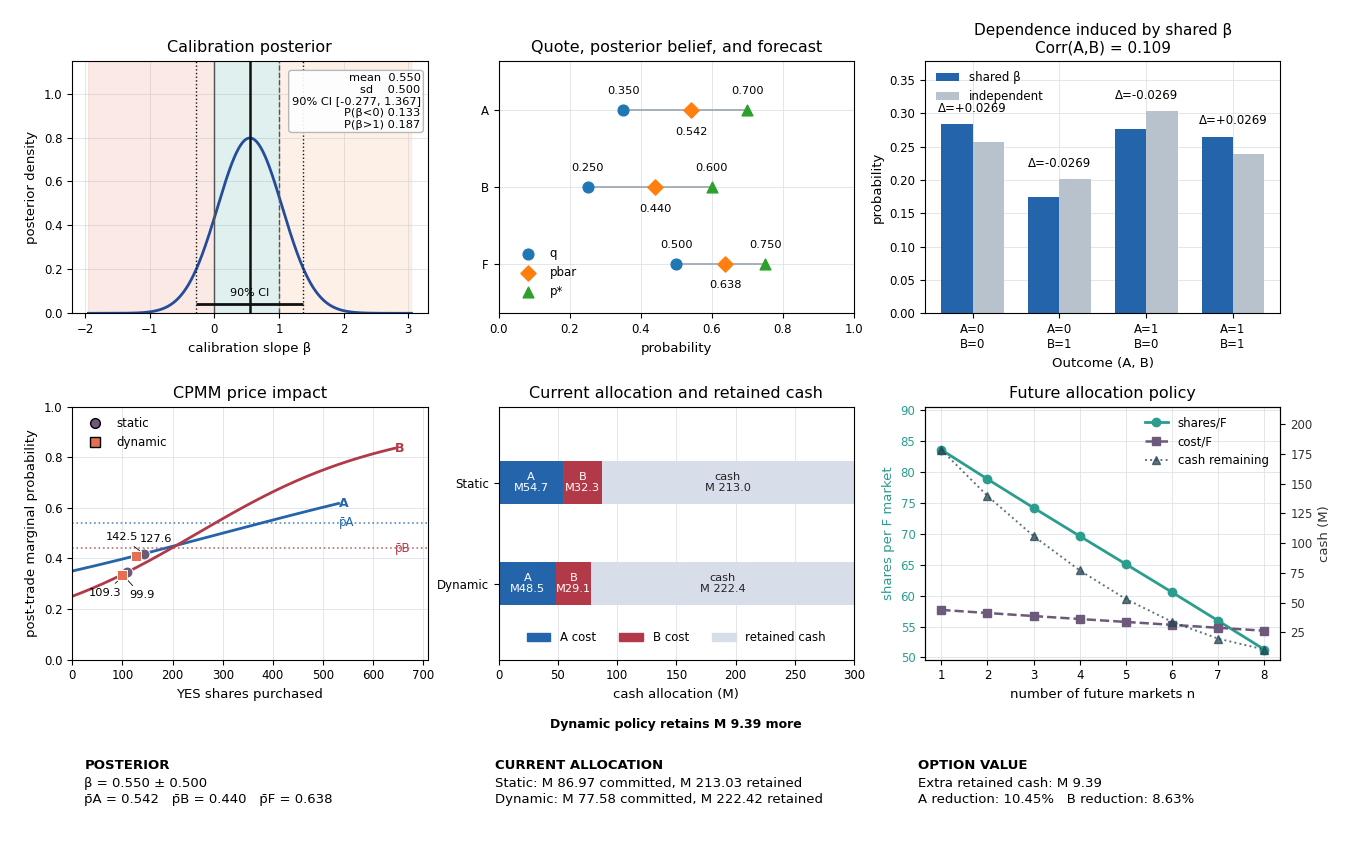
\includegraphics[width=\textwidth]{article001.png}
\caption{Numerical summary of the shared-slope specialization. The top row shows the posterior over the shared slope, the market quotes, raw forecasts, posterior predictive means, and the dependence induced between A and B. The bottom row shows exact CPMM price impact, static and dynamic current allocations, and the optimal second-stage policy as the number of future F markets varies. All values correspond to Eqs.~\eqref{eq:example-static}--\eqref{eq:stage-one} and Tables~\ref{tab:markets}--\ref{tab:future-policy}.}
\label{fig:numerical-dashboard}
\end{figure*}

\section{Implementation Procedure}
A practical system can implement the model in the following sequence.
\begin{enumerate}
\item Produce and store an object-level forecast, the market snapshot, the reasoning trace, and diagnostics $x_i$. Record which evidence is plausibly public or already represented in the market.
\item Index learning data by resolved event. Multiple forecast snapshots for one event must share one outcome likelihood, as in Eq.~\eqref{eq:event-level-likelihood}.
\item Fit a hierarchical model for latent incremental log Bayes factors, task-specific reasoning noise, shared reliability states, and important failure modes. Use correlated outcome factors for nested or causally related markets.
\item Read the complete execution state, including pools, weights, fees, limit orders, balances, and existing positions. Pin the simulator to a source revision and test simulated fills against realized platform fills.
\item Generate the joint posterior predictive distribution of unresolved and candidate outcomes. For large portfolios, use posterior simulation, factor approximations, or scenario reduction rather than enumerating all $2^m$ outcomes.
\item Estimate the marked arrival intensity from opportunity timestamps and marks. Test the Poisson assumption and use a more general point process if arrival clustering or inhibition is material.
\item Solve the signed static portfolio problem when future opportunities are negligible. Otherwise solve the arrival-only model when positions are held, or a receding-horizon approximation to the impulse-control problem when rebalancing is allowed.
\item Enforce worst-state positive wealth, use limit prices against stale execution, and reoptimize after fills, market movements, resolutions, or posterior changes.
\end{enumerate}

Reasoning diagnostics should be evaluated out of sample. Model agreement is informative only to the extent that the models or reasoning paths fail independently; several outputs sharing one source or premise do not constitute several independent observations.

\section{Limitations}
The first-principles relation in Eq.~\eqref{eq:bayes-factor-combination} does not eliminate modeling judgment. The agent must still specify priors and likelihoods for reasoning errors, source reliability, information overlap, market informativeness, and regime drift. Probability theory determines coherent updating conditional on those assumptions; it cannot infer an unknown information structure from $p_i^{\mathrm{raw}}$ and $q_i$ alone.

The market-as-baseline assumption can be inaccurate in thin or strategic markets. The latent market extension outlined above may be necessary when liquidity and participant information vary substantially. Similarly, conditional independence given a shared reliability state is only a baseline; real-world events often have direct causal dependence.

The dynamic equations also idealize trading opportunities and execution. Poisson arrivals are analytically convenient but may miss bursts and time-of-day effects. The quasi-variational inequality is a formal characterization, not a claim that a high-dimensional production system can be solved exactly. Approximate dynamic programming, scenario trees, or model-predictive control will normally be required.

Finally, log utility protects against ruin only when the predictive model and admissibility constraints cover relevant adverse states. Platform outages, rule changes, resolution disputes, account limits, and unmodeled tail events require explicit operational safeguards in addition to Bayesian optimization.

\section{Conclusion}
Kelly optimization is a rule for acting on beliefs, not a method for manufacturing confidence in a forecaster. A coherent prediction-market agent should therefore separate a fallible raw reasoning output from its final meta-level posterior. Treating the market as a public-information baseline yields a first-principles decomposition: posterior log odds equal market log odds plus an incremental log Bayes factor. A hierarchical model can then infer that evidential contribution from reasoning outputs, diagnostics, historical resolutions, and shared failure states.

The resulting joint posterior predictive distribution combines naturally with exact AMM execution and expected-log portfolio choice. Task-specific uncertainty produces position-specific caution; shared uncertainty produces dependence; existing holdings permit reductions and reversals; and future opportunities give cash an option value. Ordinary Kelly is recovered only in the special case of one frictionless market, a known final probability, no existing portfolio, and no material future decisions. Fractional-Kelly-like behavior may emerge, but it is an output of the model rather than an input.

\appendices
\section{Sum-to-One Multiple-Choice CPMM Execution}
Consider $J\geq2$ mutually exclusive and exhaustive outcomes with indicators $Y_j$ satisfying
\begin{equation}
\sum_{j=1}^{J}Y_j=1.
\end{equation}
The reviewed Manifold mechanism maintains one symmetric binary CPMM for each answer, with pools $(y_j,n_j)$, invariant $y_jn_j=k_j^2$, and probability
\begin{equation}
q_j=\frac{n_j}{y_j+n_j}.
\end{equation}
The pools are coupled by $\sum_j q_j=1$ \cite{manifold-arbitrage}.

Let $K_j^{\mathrm{Y}}(s)$ and $K_j^{\mathrm{N}}(s)$ be the fee-free binary costs. The complete-set identities are
\begin{align}
\sum_{j\neq i}(1-Y_j)&=(J-2)+Y_i,\\
\sum_{j\neq i}Y_j&=1-Y_i.
\end{align}
For a target of $s$ YES shares in answer $i$, synthesize $u$ shares through NO purchases in all complementary answers:
\begin{equation}
K_i^{\mathrm{Y,mc}}(s)
=
\min_{0\leq u\leq s}
\left[
K_i^{\mathrm{Y}}(s-u)
+
\sum_{j\neq i}K_j^{\mathrm{N}}(u)
-(J-2)u
\right].
\label{eq:mc-yes}
\end{equation}
At an interior optimum,
\begin{equation}
-q_i'+\sum_{j\neq i}(1-q_j')-(J-2)
=
1-\sum_jq_j'=0.
\end{equation}
Similarly,
\begin{equation}
K_i^{\mathrm{N,mc}}(s)
=
\min_{0\leq u\leq s}
\left[
K_i^{\mathrm{N}}(s-u)
+
\sum_{j\neq i}K_j^{\mathrm{Y}}(u)
\right],
\label{eq:mc-no}
\end{equation}
whose interior first-order condition is $\sum_jq_j'-1=0$. Under convex elementary cost curves, these are one-dimensional convex problems, and the envelope theorem gives marginal costs $q_i'$ and $1-q_i'$.

At creation, a sum-to-one market with total ante $A$ and $J$ answers uses
\begin{equation}
y_j=\frac{A}{2},
\qquad
n_j=\frac{A}{2(J-1)},
\qquad
q_j=\frac{1}{J},
\end{equation}
which also satisfies $y_j+(J-1)n_j=A$ \cite{manifold-contract}.

When a new answer is split from an Other bucket, old YES shares in Other acquire YES exposure to both the new answer and residual Other, while old NO shares are converted into YES shares in the previously named answers. The source rebuilds the relevant pools, restores the probability sum through arbitrage, and cancels limit orders on the old Other bucket \cite{manifold-answer}.

The payoff decomposition remains valid with fees and limit orders, but the execution objective must reproduce the platform's actual allocation of fees across direct, complementary, and redemption legs. It is not generally sufficient to add independently fee-inclusive binary cost curves.

\section{A Precision-Fusion Derivation of a Log-Odds Weight}
A different reduced-form interpretation treats the raw-agent log odds
\begin{equation}
a_i=\logit(p_i^{\mathrm{raw}})
\end{equation}
and market log odds
\begin{equation}
m_i=\logit(q_i)
\end{equation}
as noisy measurements of a latent full-information log odds $\theta_i$:
\begin{equation}
a_i=\theta_i+\varepsilon_{Ai},
\qquad
m_i=\theta_i+\varepsilon_{Mi}.
\end{equation}
Let the error variances be $\sigma_A^2$ and $\sigma_M^2$ and their covariance be $c$. Under a diffuse prior and a joint Gaussian error model,
\begin{equation}
\E[\theta_i\mid a_i,m_i]
=
m_i+\beta(a_i-m_i),
\end{equation}
where
\begin{equation}
\beta
=
\frac{\sigma_M^2-c}
{\sigma_A^2+\sigma_M^2-2c}.
\label{eq:precision-beta}
\end{equation}
For independent errors, $\beta=\sigma_M^2/(\sigma_A^2+\sigma_M^2)$. This gives a relative-precision derivation of log-odds weighting. It is less epistemically literal than the incremental-evidence model because forecasts are posteriors based on partly overlapping information, not ordinarily repeated measurements of one physical scalar. Nevertheless, Eq.~\eqref{eq:precision-beta} clarifies why correlated errors reduce the value of apparent agreement.

\begin{thebibliography}{00}

\bibitem{kelly1956}
J. L. Kelly, Jr., ``A new interpretation of information rate,'' \emph{Bell System Technical Journal}, vol. 35, no. 4, pp. 917--926, 1956.

\bibitem{coverthomas2006}
T. M. Cover and J. A. Thomas, \emph{Elements of Information Theory}, 2nd ed. Hoboken, NJ, USA: Wiley, 2006.

\bibitem{maclean2011}
L. C. MacLean, E. O. Thorp, and W. T. Ziemba, Eds., \emph{The Kelly Capital Growth Investment Criterion: Theory and Practice}. Singapore: World Scientific, 2011.

\bibitem{hanson2007}
R. Hanson, ``Logarithmic market scoring rules for modular combinatorial information aggregation,'' \emph{Journal of Prediction Markets}, vol. 1, no. 1, pp. 3--15, 2007.

\bibitem{chenpennock2007}
Y. Chen and D. M. Pennock, ``A utility framework for bounded-loss market makers,'' in \emph{Proc. 23rd Conf. Uncertainty in Artificial Intelligence}, 2007, pp. 49--56.

\bibitem{cox1958}
D. R. Cox, ``Two further applications of a model for binary regression,'' \emph{Biometrika}, vol. 45, nos. 3--4, pp. 562--565, 1958.

\bibitem{dawid1982}
A. P. Dawid, ``The well-calibrated Bayesian,'' \emph{Journal of the American Statistical Association}, vol. 77, no. 379, pp. 605--610, 1982.

\bibitem{kahn2012}
J. M. Kahn, ``A generative Bayesian model for aggregating experts' probabilities,'' arXiv:1207.4144, 2012.

\bibitem{satopaa2015}
V. A. Satop\"a\"a, S. T. Jensen, R. Pemantle, and L. H. Ungar, ``Partial information framework: Model-based aggregation of estimates from diverse information sources,'' arXiv:1505.06472, 2015.

\bibitem{lichtendahl2017}
K. C. Lichtendahl, Jr., Y. Grushka-Cockayne, V. R. R. Jose, and R. L. Winkler, ``Bayesian ensembles of binary-event forecasts: When is it appropriate to extremize or anti-extremize?'' arXiv:1705.02391, 2017.

\bibitem{babichenko2018}
Y. Babichenko and D. Garber, ``Learning of optimal forecast aggregation in partial evidence environments,'' arXiv:1802.07107, 2018.

\bibitem{daleyvere2003}
D. J. Daley and D. Vere-Jones, \emph{An Introduction to the Theory of Point Processes, Volume I: Elementary Theory and Methods}, 2nd ed. New York, NY, USA: Springer, 2003.

\bibitem{davis1993}
M. H. A. Davis, \emph{Markov Models and Optimization}. London, U.K.: Chapman \& Hall, 1993.

\bibitem{oksendal2019}
B. \O ksendal and A. Sulem, \emph{Applied Stochastic Control of Jump Diffusions}, 3rd ed. Cham, Switzerland: Springer, 2019.

\bibitem{manifold-cpmm}
Manifold Markets, ``Binary CPMM calculation and execution source,'' \texttt{common/src/calculate-cpmm.ts}, commit \texttt{c431f5e}, Jul. 12, 2026. [Online]. Available: \url{https://github.com/manifoldmarkets/manifold/blob/c431f5e923f301d2af3c8219a700f0abcea722fb/common/src/calculate-cpmm.ts}

\bibitem{manifold-contract}
Manifold Markets, ``Contract initialization source,'' \texttt{common/src/new-contract.ts}, commit \texttt{c431f5e}, Jul. 12, 2026. [Online]. Available: \url{https://github.com/manifoldmarkets/manifold/blob/c431f5e923f301d2af3c8219a700f0abcea722fb/common/src/new-contract.ts}

\bibitem{manifold-fees}
Manifold Markets, ``Fee calculation source,'' \texttt{common/src/fees.ts}, commit \texttt{c431f5e}, Jul. 12, 2026. [Online]. Available: \url{https://github.com/manifoldmarkets/manifold/blob/c431f5e923f301d2af3c8219a700f0abcea722fb/common/src/fees.ts}

\bibitem{manifold-arbitrage}
Manifold Markets, ``Multiple-choice CPMM arbitrage source,'' \texttt{common/src/calculate-cpmm-arbitrage.ts}, commit \texttt{c431f5e}, Jul. 12, 2026. [Online]. Available: \url{https://github.com/manifoldmarkets/manifold/blob/c431f5e923f301d2af3c8219a700f0abcea722fb/common/src/calculate-cpmm-arbitrage.ts}

\bibitem{manifold-answer}
Manifold Markets, ``Multiple-choice answer creation and Other conversion source,'' \texttt{backend/api/src/create-answer-cpmm.ts}, commit \texttt{c431f5e}, Jul. 12, 2026. [Online]. Available: \url{https://github.com/manifoldmarkets/manifold/blob/c431f5e923f301d2af3c8219a700f0abcea722fb/backend/api/src/create-answer-cpmm.ts}

\end{thebibliography}

\end{document}
